\chapter{Häufige Fragen und Probleme mit Latex}

Im Laufe der Arbeit mit Latex stoßen Schüler immer wieder auf sehr ähnliche Probleme und Fehler. 
Dieses Kapitel stellt eine Sammlung der häufigsten Probleme und Fehler dar und soll als erste Anlaufstelle zur Problemlösung dienen.

\subsubsection*{Umlaute (ö, Ö, ü, Ü, ä, A, ß, ...) werden im erzeugten PDF nicht korrekt dargestellt oder erzeugen Fehler beim Erzeugen des PDFs.}
Dieser Fehler wird fast immer durch eine falsche Zeichenkodierung\footnote{\url{https://de.wikipedia.org/wiki/Zeichenkodierung}} der Textdatei erzeugt. 
Die Vorlage erwartet durchgehend mit UTF-8\footnote{\url{https://de.wikipedia.org/wiki/UTF-8}} erzeugte Textdateien. 
Leider erzeugen einige Editoren bzw. Betriebssysteme standardmäßig keine UTF-8 Textdateien. Abhilfe schafft ein einfaches neu speichern der Textdatei als UTF-8. 
Die Zeichenkodierung kann bei den meisten Editoren im \textit{Speichern unter} Dialog ausgewählt werden wie in Abbildung \ref{fig:speichernunter} dargestellt.

\begin{figure}
\centering
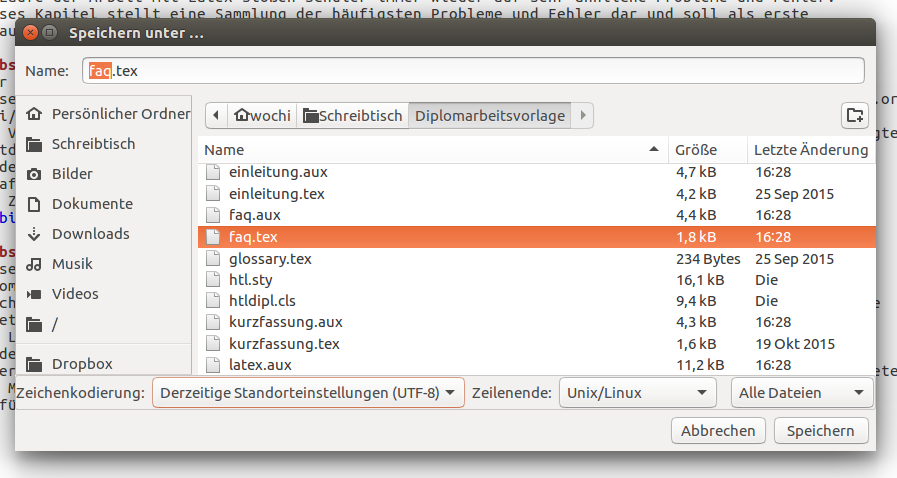
\includegraphics[width=.85\textwidth]{SpeichernUnter}
\caption{Speichern Unter Dialog mit der Auswahlmöglichkeit der Zeichenkodierung}
\label{fig:speichernunter}
\end{figure}

\subsubsection*{Beim Erzeugen des PDFs kommt eine Fehlermeldung das Paket XYZ.sty fehlt.}
Dieser Fehler hängt von der verwendeten Latex-Installation ab. Bei Miktex können fehlende Pakete automatisch nachinstalliert werden. 
Manchmal funktioniert diese Automatik jedoch nicht. In diesem Fall ist es am Einfachsten die fehlende Pakete im Miktex-Manager manuell zu installieren. 
Bei Linux und anderen Betriebssystemen kann die Latex-Umgebung meist als Full-Install installiert werden. Hier werden alle verfügbaren Pakete installiert. 
Alternativ kann man mit Google ermitteln welches Installationspaket\footnote{Übersicht der Latex-Pakete für Mac \url{https://trac.macports.org/wiki/TeXLivePackages}} die benötigen XYZ.sty Dateien zur Verfügung stellt.

\subsubsection*{Das Inhaltsverzeichnis, Glossar, Literaturverzeichnis, ... wird nicht mehr angezeigt.}
Wärend die einzelnen Kapitel der Vorlage in der Datei \textit{\_Diplomarbeitsvorlage.tex} problemlos gegen die eigenen Kapitel ausgetauscht werden können, sind die anderen Befehle in dieser Datei kritisch für ein funktionieren der Vorlage. Wurde hier aus Versehen eine falsche Zeile gelöscht oder verändert, kann dies unerwartete Auswirkungen haben. In dem Fall am Besten die eigene \textit{\_Diplomarbeitsvorlage.tex} mit der aus der Vorlage vergleichen und gegebenenfalls eigene Änderungen vorübergehen zurück nehmen bis der Fehler gefunden ist.